\documentclass{article}

\usepackage{microtype}
\usepackage{tabu}
\usepackage{graphicx}
\usepackage[hidelinks]{hyperref}
\usepackage{amsmath}
\usepackage{mathtools}

\title{Project: Kinematics Pick \& Place}
\author{Grace Livingston}

\newcommand{\halfpi}{\frac{\pi}{2}}

\extrarowsep=1pt
\begin{document}
\maketitle
\tableofcontents

\newpage

\section{Kinematic Analysis}

I looked at the parameters in the \texttt{kr210.urdf.xacro} file and
extracted the position and pose angles for each link and joint.
The schematics of the joints are:

\begin{table}[h]
    \begin{center}
        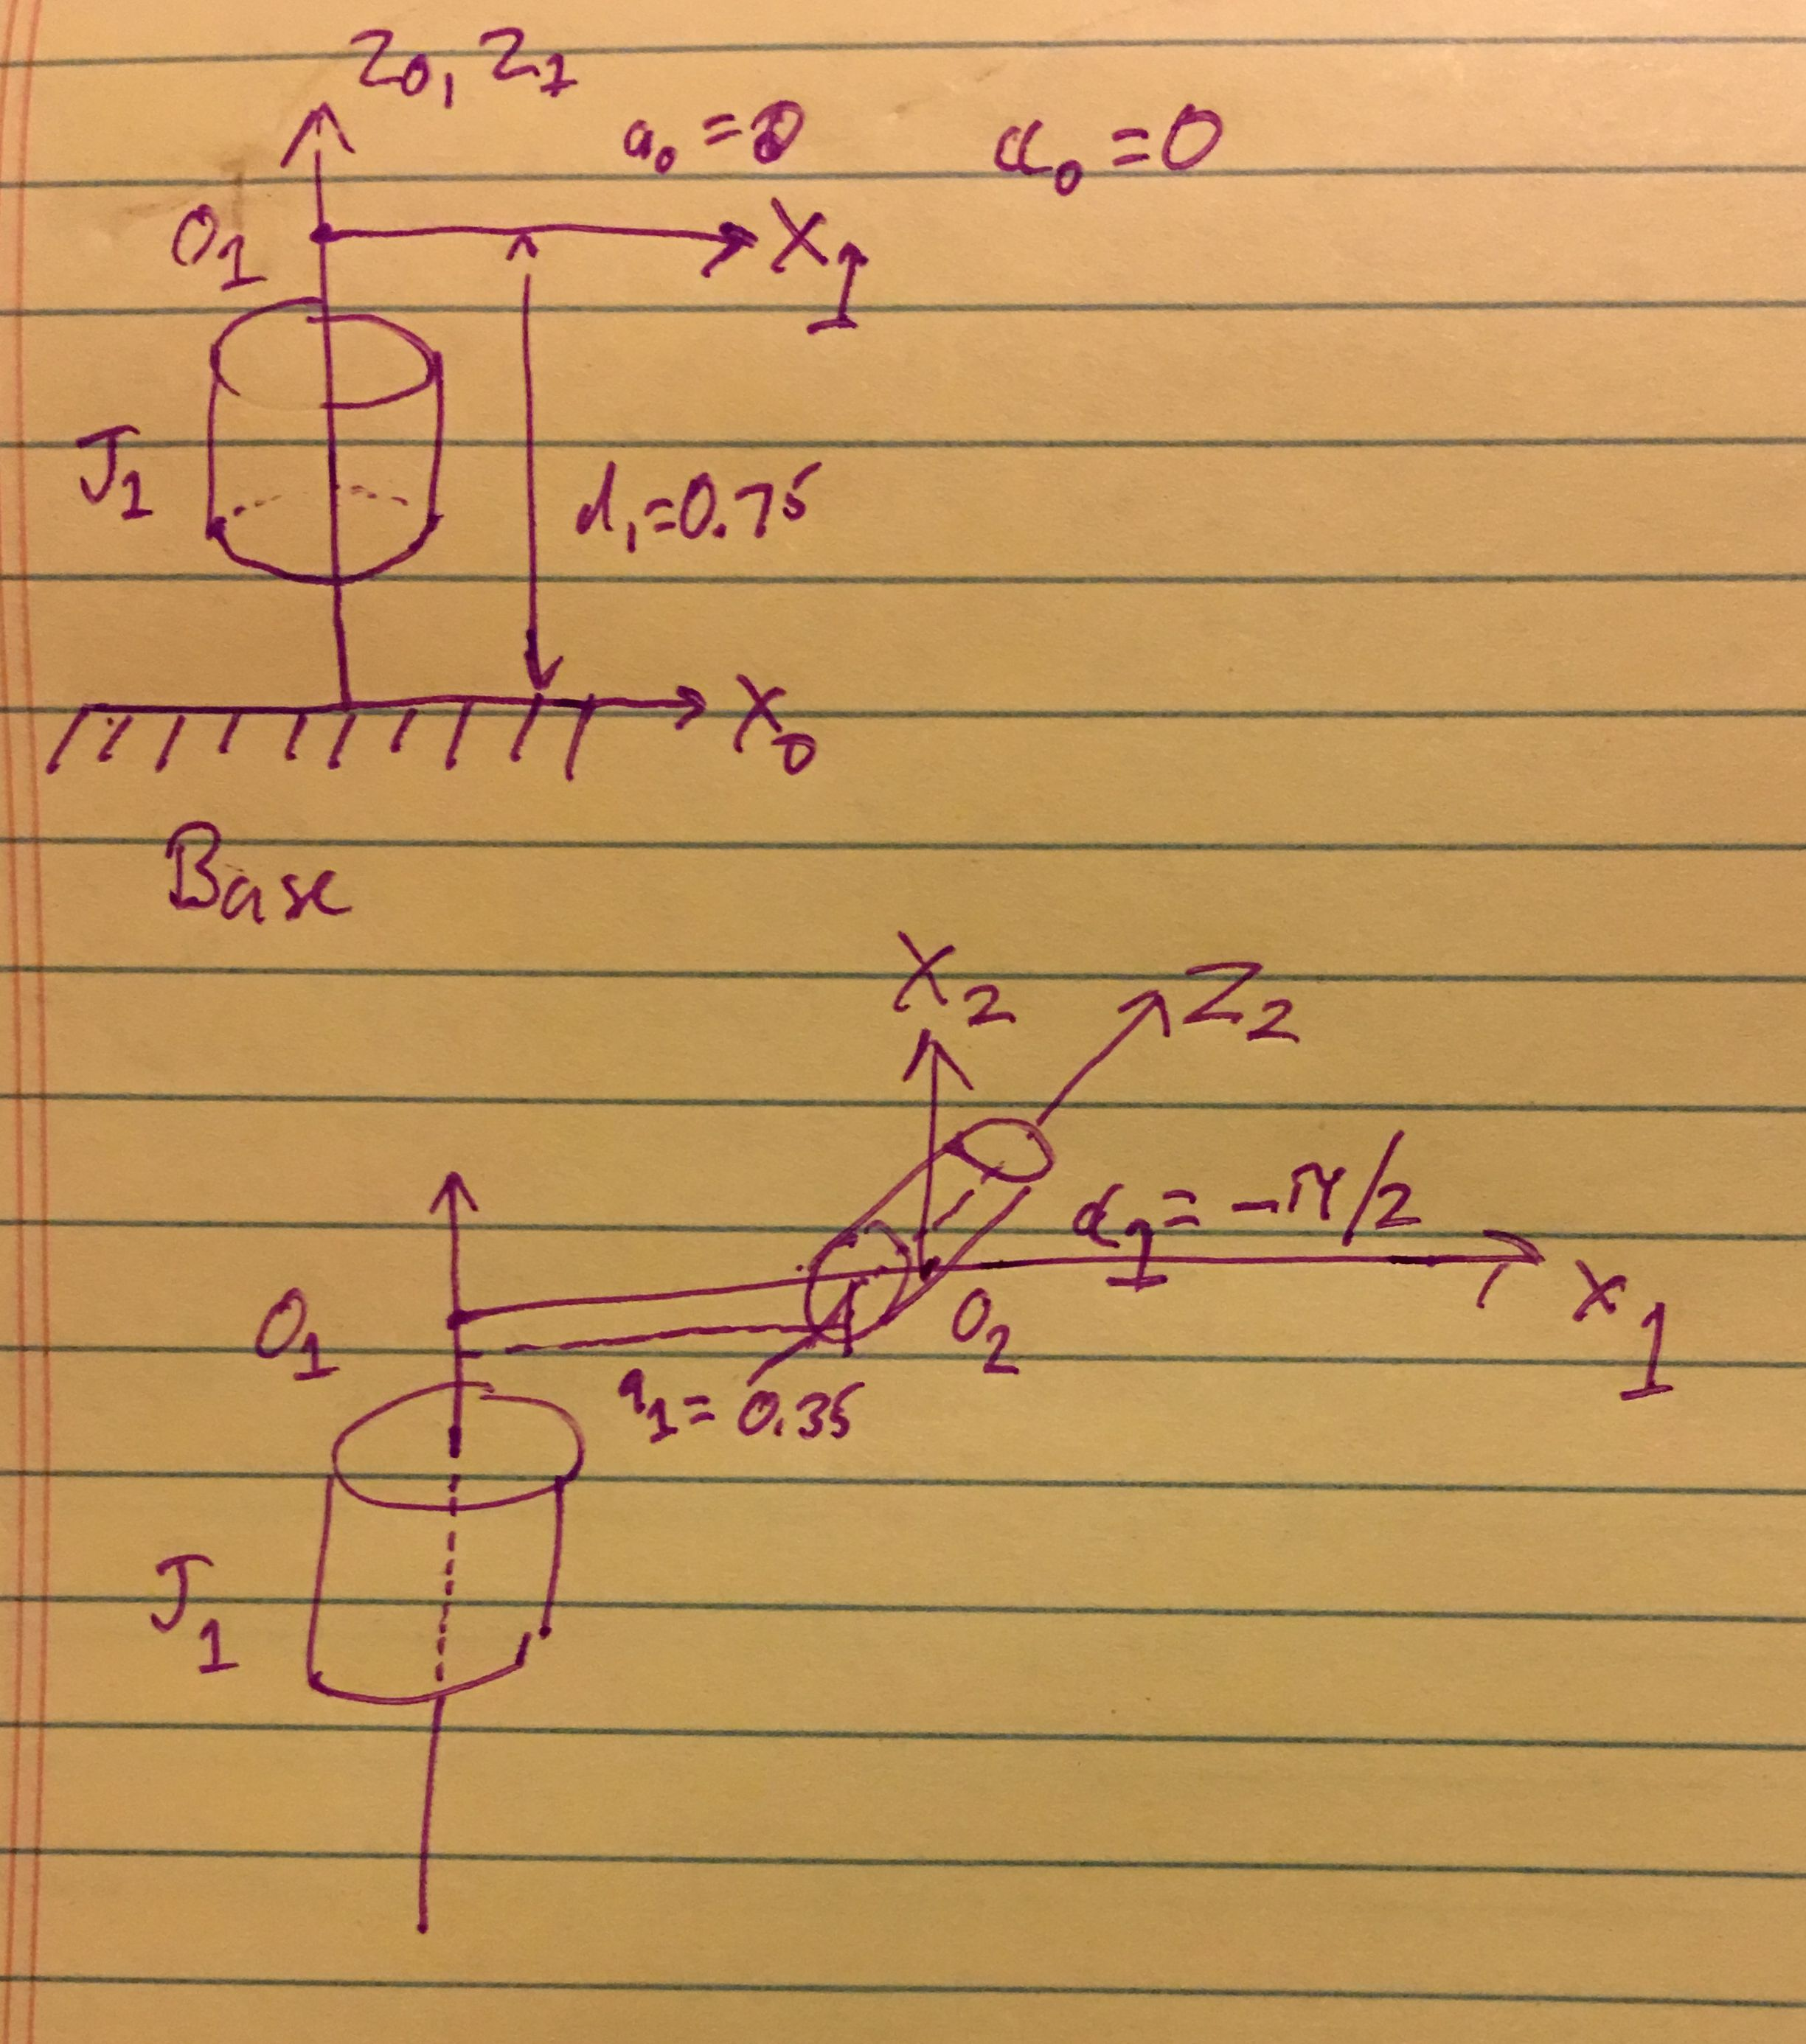
\includegraphics[width=0.5\textwidth]{misc_images/sch1.jpeg}
    \end{center}
    \caption{$J_1 - J_2$}
\end{table}

\begin{table}[h]
    \begin{center}
        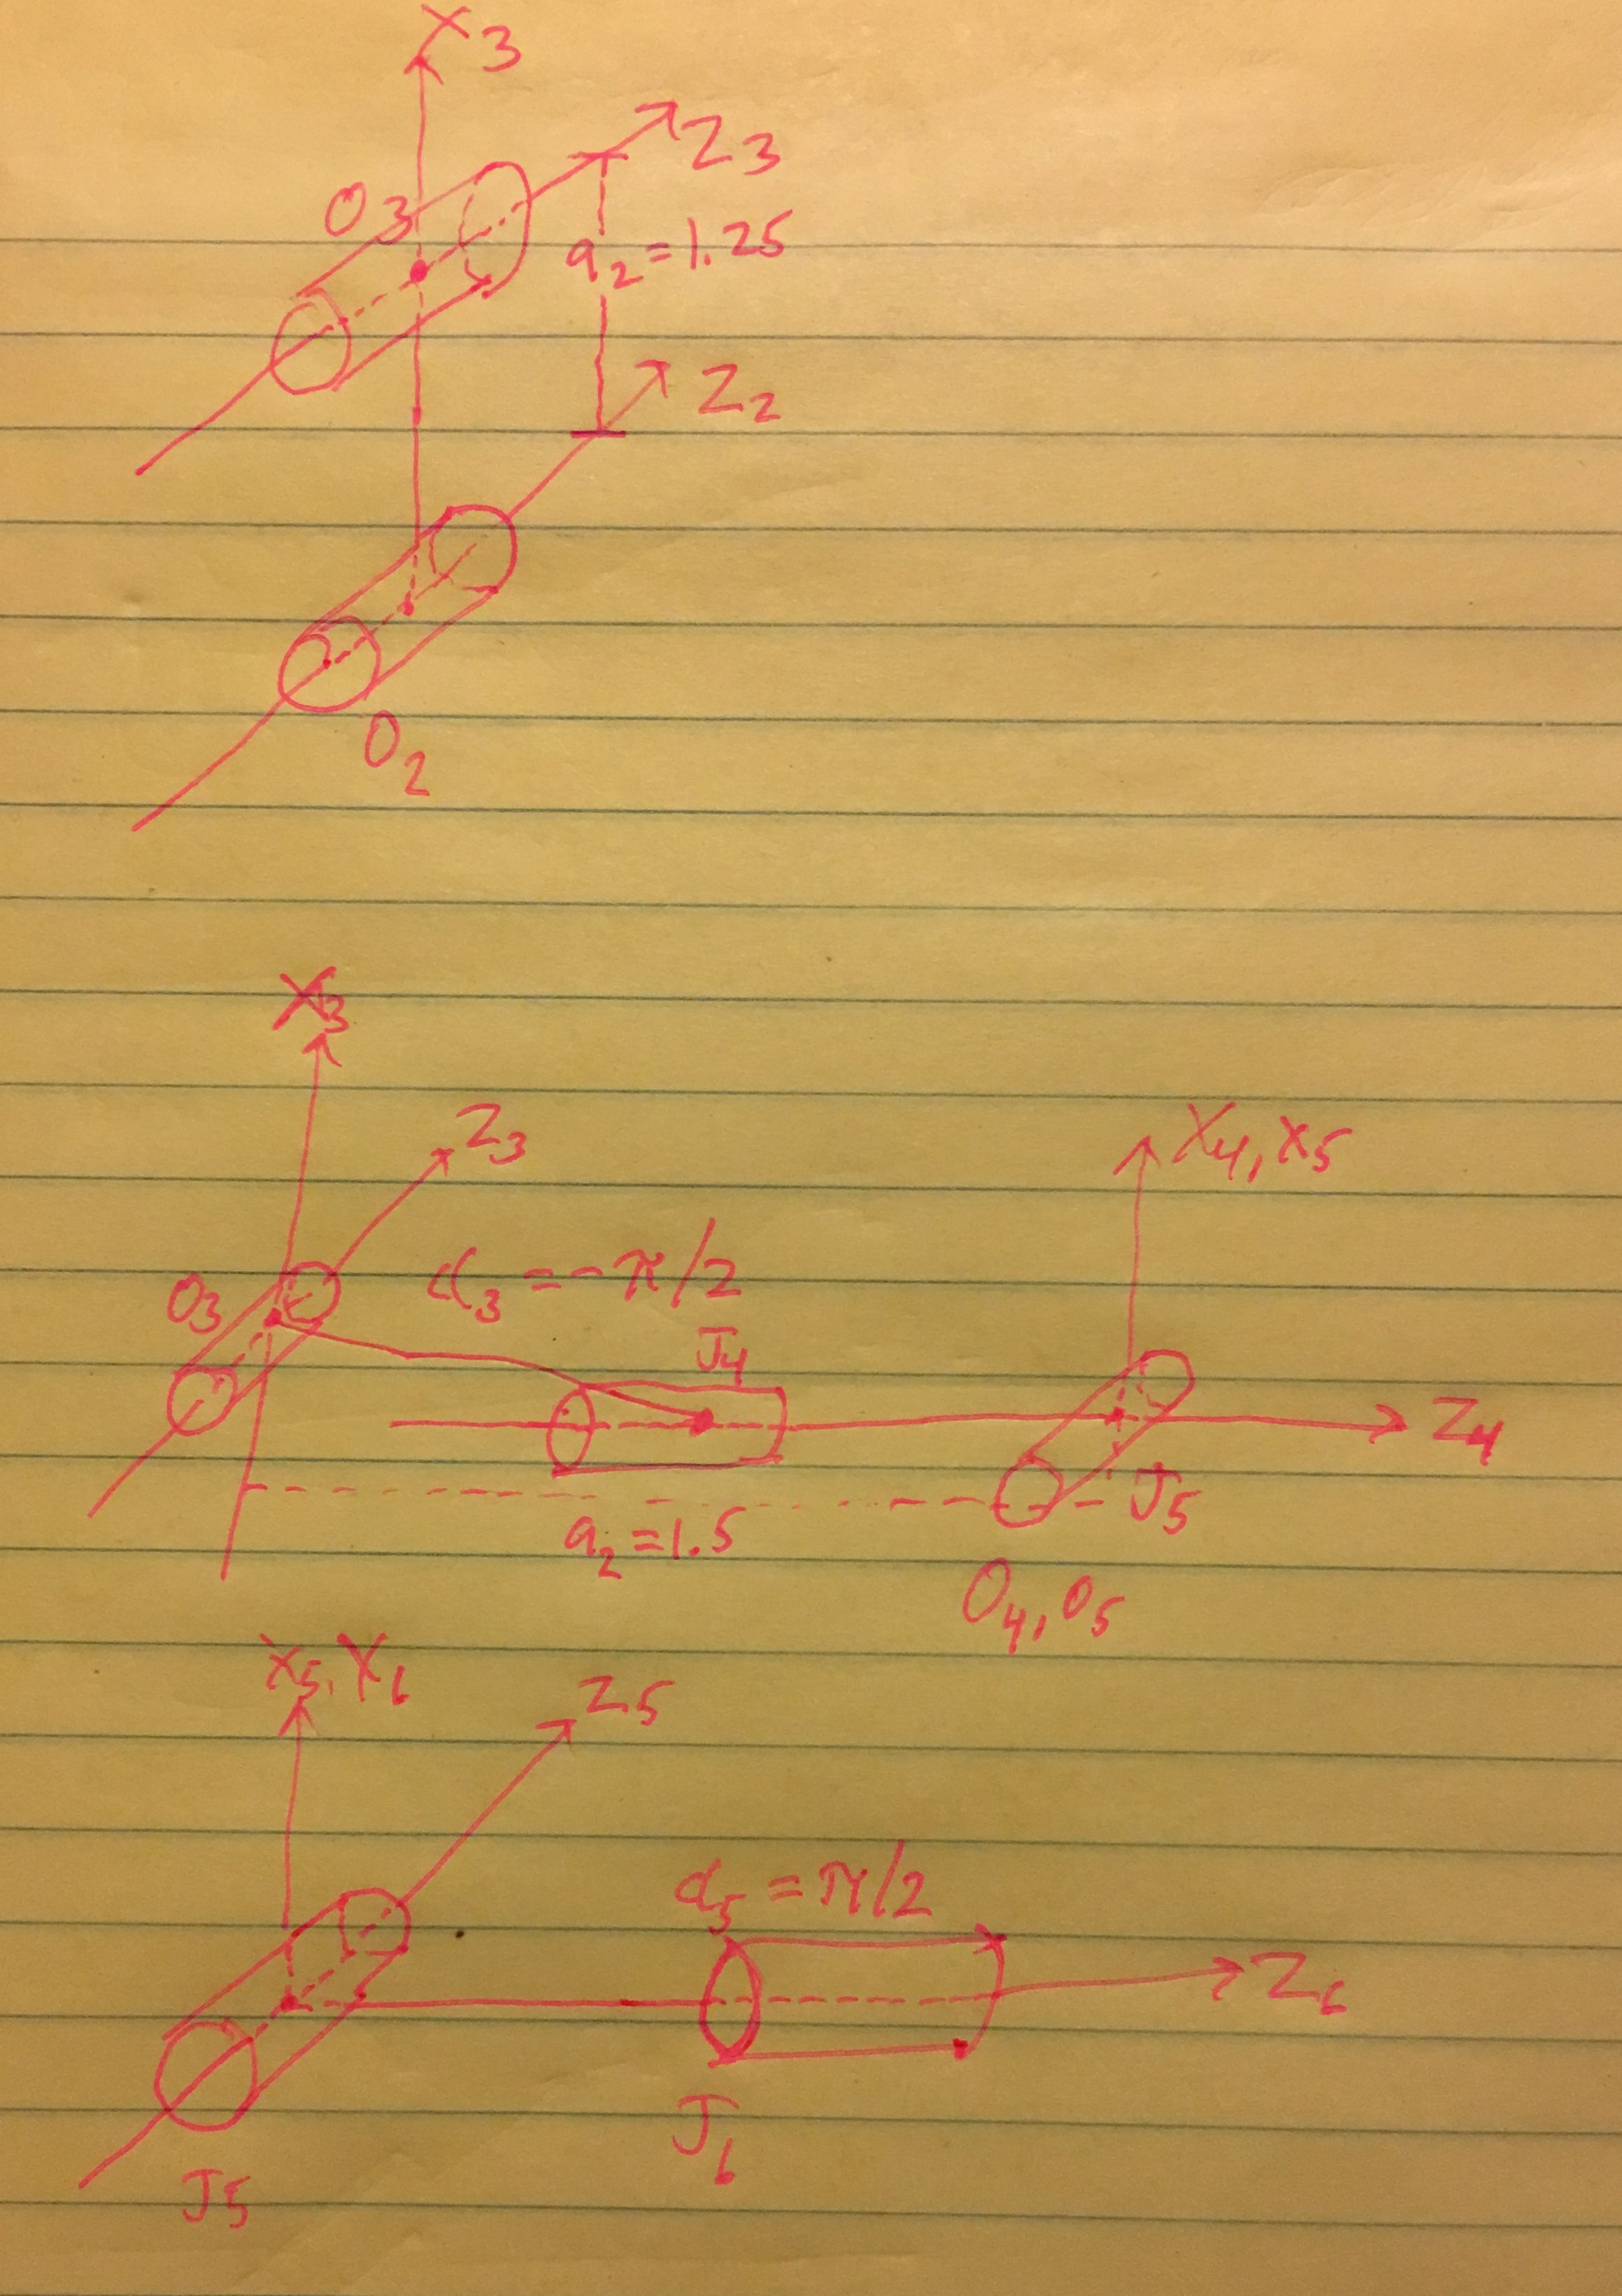
\includegraphics[width=0.5\textwidth]{misc_images/sch2.jpeg}
    \end{center}
    \caption{$J_3 - J_6$}
\end{table}

\newpage

\section{DH Table}

\begin{center}
    \begin{small}
\begin{tabu} to 0.75\linewidth {|[1pt]X[2$]|[1pt]X[1$]|X[1$]|X[1$]|X[1$]|[1pt]}
  \tabucline[1pt]-
  Link & \alpha_{i-1} & a_{i-1} & d_{i-1} & \Theta_{i-1} \\
  \tabucline[1pt]-
  \everyrow{\tabucline-}
  T_{0,1}: 0 \rightarrow 1 & 0.00 & 0.00 & 0.75 & \Theta_1 \\
  T_{1,2}: 1 \rightarrow 2 & -\halfpi & 0.35 & 0.00 & \Theta_2 - \frac{\pi}{2} \\
  T_{2,3}: 2 \rightarrow 3 & 0.00 & 1.25 & 0.00 & \Theta_3 \\
  T_{3,4}: 3 \rightarrow 4 & -\halfpi & -0.054 & 1.50 & \Theta_4 \\
  T_{4,5}: 4 \rightarrow 5 & \halfpi & 0.00 & 0.00 & \Theta_5 \\
  T_{5,6}: 5 \rightarrow 6 & -\halfpi & 0.00 & 0.00 & \Theta_6 \\\everyrow{}
  T_{6,EE}: 6 \rightarrow {EE} & 0.00 & 0.00 & 0.303 & \Theta_{EE} \\
  \tabucline[1pt]-
\end{tabu}
\end{small}
\end{center}


\section{Foward Kinematics}

DH uses four transforms: $R_X, D_X, R_Z, D_Z$
\begin{equation}
    \prescript{i-1}{i}T = R_X(\alpha_{i-1})D_X(\alpha_{i-1})R_Z(\theta_i)D_Z({d_i})
\end{equation}

Using above DH parameter table, we can create individual transforms
between various links:

\begin{equation}
    \prescript{i-1}{i}T = \begin{pmatrix}
        \cos(\theta) & -\sin(\theta) & 0 & a \\
        \sin(\theta)\cos(\alpha) & -\sin(\alpha) & -d\sin(\alpha) \\
        \sin(\theta)\sin(\alpha) & \cos(\theta)\sin(\alpha) &
        \cos(\alpha) & d\cos(\alpha) \\
        0 & 0 & 0 & 1
    \end{pmatrix}
\end{equation}

In Python, this is the \texttt{TF\_Mat} function. It’s used to define
the individual transformation matrices \texttt{TF\_0\_1} through
\texttt{TF\_6\_7}. These are then composed to the Homogeneous Transform
for the entire arm \texttt{TF\_0\_7}.

The translational correction from URDF to DH parameters
(\texttt{R\_corr}) is applied, the Euler angles are extracted and
roll, pitch, and yaw matrices computed (\texttt{ROT\_x},
\texttt{ROT\_y}, \texttt{ROT\_z}), and the correction from Gazebo
applied (\texttt{ROT\_corr}), giving us the rotation matrix for the
End Effector \texttt{ROT\_EE}.

\section{Inverse Kinematics}

Given an end effetor position, calculate the joint angles required.
There are two approaches: numeric and closed-form. Since this robot
satisfies the requirements for the closed-form solution, I opted for
the closed-form. The last three joints ($J_4, J_5, J_6$) share
a common intersection ($J_5$), if we calculate the position of the
wrist center (${WC}$), we can then calculate the orientation of the
final three joints independently.

Each position provided consists of the position and orientation of the
End Effector, the \texttt{pose}. The orientation is provided as
a quaternion so we convert that to Euler angles.

The Euler angles can then be used to find the rotation matrix with the
correction applied:

\begin{equation}
    R_{rpy} = R_{corr}(R_y(Z, y)R_p(Y, p)R_r(X, r))
\end{equation}

This is then the rotation component of the Homogenous Transform:

\begin{equation}
    \begin{bmatrix}
        \mathbf{l_x} & \mathbf{m_x} & \mathbf{n_x} & p_x \\
        \mathbf{l_y} & \mathbf{m_y} & \mathbf{n_y} & p_y \\
        \mathbf{l_z} & \mathbf{m_z} & \mathbf{n_z} & p_z \\
        0 & 0 & 0 & 1
    \end{bmatrix}
\end{equation}

The vectors $\mathbf{l}, \mathbf{m}, \mathbf{n}$
represent the End Effector position along the local $X, Y, Z$
frame. If $\mathbf{n}$ is the vector along the gripper link axis, the
position of the center of the wrist $X_{WC}$ is:

\begin{align}
  D &= d_6 + d_7 \\
  W_x &= p_x - D \times n_x \\
  W_y &= p_y - D \times n_y \\
  W_z &= p_z - D \times n_z
\end{align}

We can project $W_z$ onto the ground plane to find $\theta_1$:

\begin{equation}
    \theta_1 = \arctan(W_y, W_x)
\end{equation}

Then we can calculate $\theta_2$ and $\theta_3$ by completing the
triangle  $\bigtriangleup A = d4, B, C = a2$:

\begin{align}
  A &= \sqrt{W_x^2 + W_y^2} - a_1 \\
  C &= W_z - d_1 \\
  B &= \sqrt{A^2 + C^2} \\
  a &= \arccos(\frac{B^2 + C^2 - A^2}{2BC}) \\
  b &= \arccos(\frac{A^2 + C^2 - B^2}{2AC}) \\
  c &= \arccos(\frac{A^2 + B^2 - C^2}{2AB}) \\
  \theta_2 &= \frac{\pi}{2} - a - \arctan(W_z - 0.75, \sqrt{W_x^2 + W_y^2} - 0.35) \\
  \theta_3 &= \frac{\pi}{2} - (b + 0.36)
\end{align}

Now we can find the values of $\theta_4, \theta_5, \theta_6$.
These are coincident on the wrist center $\mathbf{W}$,
and they are orthogonal. The full $R_{EE}$
Matrix is a linear combination of $R_{0} \dots R_{EE}$.
Since we have $R_{0} \dots R_{3}$,
and since $R_{4} \dots R_{6}$
are orthogonal, we can find them by multiplying $R_{EE}$
by the inverse of $R_{0} \dots R_{3}$ and then decomposing
$R_{4\dots6}$ into $R_4, R_5, R_6$:

\begin{align}
  R &= R_{0\dots3} \times R_{4\dots6} \\
  R_ {3\dots6} &= R_{0\dots3}^T \times R
\end{align}

The best solution to $R_{3\dots6}$ can be determined from the quadrant
of $\theta_5$.

\end{document}